
\documentclass{ecpreport-publicv1}
\usepackage{draftwatermark}
\usepackage{wrapfig}
\usepackage{subfig}
\usepackage{xcolor,colortbl}
\usepackage{array}
\newcolumntype{L}[1]{>{\raggedright\let\newline\\\arraybackslash\hspace{0pt}}m{#1}}
\definecolor{Gray}{gray}{0.85}
\definecolor{LightCyan}{rgb}{0.88,1,1}

\newcolumntype{g}{>{\columncolor{Gray}}c}
\newcolumntype{w}{>{\columncolor{white}}c}
\newcolumntype{y}{>{\columncolor{LightCyan}}c}

%\usepackage{subcaption}
%\usepackage{graphicx}
\newcommand{\pmr}{Programming Models \& Runtimes}
\newcommand{\tools}{Development Tools}
\newcommand{\mathlibs}{Mathematical Libraries}
\newcommand{\dataviz}{Data \& Visualization}
\newcommand{\ecosystem}{SW Ecosystem \& Delivery}
\newcommand{\stid}[1]{{\texttt{WBS 2.3.{#1}}}}
\usepackage[framemethod=TikZ,backgroundcolor=gray!40,shadow=true,roundcorner=8pt]{mdframed}
\usetikzlibrary{shadows}
\usepackage{hyperref}
\hypersetup{
	colorlinks,
	citecolor=blue,
	filecolor=blue,
	linkcolor=blue,
	urlcolor=blue
}



%%---------------------------------------------------------------------------%%
%% VARIABLES
%%---------------------------------------------------------------------------%%
\author{Michael A.~Heroux, Director ECP ST
  \and Jonathan Carter, Deputy Director ECP ST
  \and Rajeev Thakur, Programming Models \& Runtimes Lead
  \and Jeffrey Vetter, Development Tools Lead
  \and Lois Curfman McInnes, Mathematical Libraries Lead
  \and James Ahrens, Data \& Visualization Lead
  \and J.~Robert Neely, Software Ecosystem \& Delivery Lead}
\title{ECP Software Technology Capability Assessment Report}
%\date{\today}
\date{January 1, 2019}
%\wbs{2.3}
\id{ECP-RPT-ST-0001-2019}
\reportnum{ECP-RPT-ST-0001-2019}

\submitter{Michael A.~Heroux}

%\concurrence{Douglas Kothe}
%\concurrenceorg{ECP Director}
%
%\approver{Dan Hoag}
%\approverorg{Federal Project Administrator}

%%---------------------------------------------------------------------------%%
%% FRONT MATTER
%%---------------------------------------------------------------------------%%

\begin{document}
\frontmatter

%%---------------------------------------------------------------------------%%
%% REVISION LOG

\begin{revlog}

  1.0 & July 1, 2018 & \textit{ECP ST Capability Assessment Report } \\\hline
  1.5 & \today & New revision--DRAFT \\\hline
\end{revlog}

%%---------------------------------------------------------------------------%%
% EXECUTIVE SUMMARY

\input{abstract}


\tableofcontents
\listoffigures
\listoftables

%%---------------------------------------------------------------------------%%
% MAIN DOCUMENT
%%---------------------------------------------------------------------------%%

\mainmatter
\input{Introduction}

\newpage
\section{ECP ST Technical Areas}
\input{projects/2.3.1-PMR/2.3.1-PMR}
\input{projects/2.3.2-Tools/2.3.2-Tools}
\input{projects/2.3.3-MathLibs/2.3.3-MathLibs}
\input{projects/2.3.4-DataViz/2.3.4-DataViz}
\input{projects/2.3.5-Ecosystem/2.3.5-Ecosystem}

\newpage
\section{ECP ST Deliverables}\label{sect:deliverables}
\input{Deliverables-Overview}
\input{Products}
\input{Standards}
\input{Design}


%%---------------------------------------------------------------------------%%
%\vspace{3in}
\clearpage
%\newpage
\section{ECP ST Project Summaries}\label{sect:project-summaries}

This section of the ECP ST Capabilities Assessment Report provides two-page summaries of each funded project.  The text provides a project overview and summarizes the key challenges, solution strategy, recent progress and next steps for the project.
\newpage
\subsection{\pmr}
This section present projects in \pmr.
\newpage
\input{projects/2.3.1-PMR/2.3.1.01-PMR-SDKs/2.3.1.01-PMR-SDKs}
\newpage
\input{projects/2.3.1-PMR/2.3.1.02-LANL-ATDM-PMR/2.3.1.02-LANL-ATDM-PMR}
\newpage
\subsubsection{\stid{1.03} LLNL ATDM Programming Models and Runtimes}


\paragraph{Overview} 
%\textit{Provide an overview of your project.  You might find that the introductory text from your Fall 2017 Project Summary \url{https://confluence.exascaleproject.org/display/1ST/Fall+2017+ECP+ST+Project+Summaries} useful as a starting draft.}
This project covers two main thrusts in programming models standards and 
runtimes for exascale supercomputing systems. The first thrust is 
programming models standards work in MPI and OpenMP. 

The Message Passing Interface Standard (MPI) is a message passing library standard based on the consensus of the MPI Forum, which has over 40 participating organizations, including vendors, researchers, software library developers, and users. The goal of the Message Passing Interface is to establish a portable, efficient, and flexible standard for message passing that will be widely used for writing message passing programs. As such, MPI is the first standardized, vendor independent, message passing library. The advantages of developing message passing software using MPI closely match the design goals of portability, efficiency, and flexibility. MPI is not an IEEE or ISO standard, but has in fact, become the ``industry standard'' for writing message passing programs on HPC platforms.

OpenMP (Open Multi-Processing) is an application programming interface (API) that supports multi-platform shared memory multiprocessing programming in C, C++, and Fortran, on most HPC platforms. To enable portable tools for performance analysis and debugging of OpenMP programs, the OpenMP Language Committee is defining application programming interfaces for tools; these interfaces are expected to be part of the OpenMP standard and supported by all OpenMP compliant implementations. There are two parts to the proposed interfaces: OMPT (a first-party API for performance tools), and OMPD (a shared-library plugin for debuggers that enables a debugger to inspect and control execution of an OpenMP program).

The other main thrust area for LLNL is the ROSE project’s work in support of 
ATDM Exascale application efforts.  
ROSE is an open source compiler infrastructure to build source-to-source program transformation and analysis tools for large-scale Fortran 77/95/2003, C, C++, OpenMP, and UPC applications. The intended users of ROSE could be either experienced compiler researchers or library and tool developers who may have minimal compiler experience. ROSE is particularly well suited for building custom tools for static analysis, program optimization, arbitrary program transformation, domain-specific optimizations, complex loop optimizations, performance analysis, and cyber-security.



\paragraph{Key  Challenges} \leavevmode \\
%\textit{Describe what is hard to do, why it is challenging.}

\textbf{ROSE.}
We will develop advanced program 
transformation and analysis to improve correctness and performance of 
RAJA codes. The research results will be communicated to RAJA maintainers to 
improve the RAJA portable programming layer. Both of these LLNL efforts 
in this area  are crucial for ECP and ASC applications to achieve portable 
performance on upcoming Exascale systems.

\textbf{MPI.}
For MPI, we focus on 
interfaces for supporting tools, including MPI\_T and MPIR, and for fault
tolerance, including Reinit. Tools for MPI are critical to ensure that
applications achieve high communication performance, and understanding
and designing fault tolerance interfaces are important for large scale
jobs on faulty systems.
The participants will follow development across the standard in
addition to the tools and fault tolerance areas. 

\textbf{OpenMP.} 
In OpenMP, our focus is on the tools interfaces 
OMPT and OMPD.  Tools are critical for application developers to understand
the correctness and performance of their codes when using OpenMP.
We will participate and monitor developments in 
all parts the standard in addition to our focus areas. 

\paragraph{Solution Strategy} \leavevmode \\
 
%\textit{Describe your basic strategy for addressing the challenges.}

\textbf{ROSE.}
The team is working to support advanced loop transformations on RAJA
code; finding loops susceptible to data races in ASC applications;
and performing performance analysis of RAJA code. ROSE improvements
will be released as open source at \url{https://github.com/rose-compiler/rose
}.

\textbf{MPI.}
LLNL staff regularly participate in regular calls and discussions for the Tools Working Group, Fault Tolerance Working Group, Sessions Working Group and attend Forum meetings that occur during the quarter.

\textbf{OpenMP.} Regularly participate in weekly OpenMP language committee calls, participate in biweekly calls of the OpenMP tools WG, email discussions on OpenMP tools interfaces (OMPD and OMPT).

\begin{figure}[htb]
        \centering
        \includegraphics[width=4in]{projects/2.3.1-PMR/2.3.1.03-LLNL-ATDM-PMR/ROSE-raja}
        \caption{\label{fig:rose-raja}\textbf{Work by ROSE team shows
performance gap analysis for RAJA with different compilers.}}
\end{figure}




\paragraph{Recent Progress} \leavevmode \\

%\textit{Describe what you have done recently.  It would be good to have some kind of figure or diagram in this section.}


\textbf{ROSE.} The team continued to improve ROSE's C++11 support 
and the ROSE-based 
tool, rajaChecker. 
The team improved rajaChecker to support patterns buried deep within control 
flows. Additionally, they improved the robustness of rajaChecker and 
significantly reduced compilation errors in a large ASC application.
The team improved the tool's debugging support by adding more detailed
execution tracing information. The debugging information was used to
find the root cause of several false negative reports, which the team 
subsequently fixed. They also added new features in rajaChecker to
collect statistics about the total number of loops analyzed and how 
many loops are lambda or regular loops.



\textbf{MPI.} The MPI participants participated in the design of new 
approaches to incorporate fault tolerance in the MPI Standard, including 
standardizing primitives to support fundamental fault-tolerance methods.  
They also worked on the MPI\_T\_Events interface for tools.
The MPI participants attended the MPI Forum meetings in 2018
and proposed new approaches to incorporate fault tolerance in the 
MPI Standard, including standardizing primitives to support fundamental 
fault-tolerance methods.

\textbf{OpenMP.} In OpenMP, 
the project members attended the OpenMP 
face-to-face meeting in Austin and worked with the Tools subcommittee 
to prepare and enact several tickets to improve OMPT and OMPD 
specifications. In particular, they improved the OMPD prototype for
NVIDIA GPUs and the clang/LLVM runtime. They also updated the OMPD
prototype runtime to be fully compliant with OpenMP 5.0.


\paragraph{Next Steps}  \leavevmode \\


\textbf{ROSE.} Continue to improve ROSE support for RAJA and ASC applications.

\textbf{MPI.} Continue to participate in MPI Forum on fault tolerance and
tools.

\textbf{OpenMP.} Continue to participate in OpenMP Standards Committee
on tools and debuggers.

\newpage
\input{projects/2.3.1-PMR/2.3.1.04-SNL-ATDM-PMR/2.3.1.04-SNL-ATDM-PMR-Kokkos}
\newpage
\input{projects/2.3.1-PMR/2.3.1.04-SNL-ATDM-PMR/2.3.1.04-SNL-ATDM-PMR-Darma}
\newpage
\input{projects/2.3.1-PMR/2.3.1.05-Global-Arrays/2.3.1.05-Global-Arrays}
\newpage
\input{projects/2.3.1-PMR/2.3.1.06-RAJA/2.3.1.06-RAJA}
\newpage
\subsubsection{\stid{1.07} Exascale MPI} \label{subsubsect:mpich}
\paragraph{Overview}

MPI has been the de facto standard programming model for HPC from the
mid 90's till today, a period where supercomputing performance
increased by six orders of magnitude.  The vast majority of DOE's
parallel scientific applications running on the largest HPC systems
use MPI.  These application codes represent billions of dollars of
investment.  Therefore, MPI must evolve to run as efficiently as
possible on Exascale systems.  Our group at Argonne developed a
high-performance, production-quality MPI implementation, called MPICH.
The focus areas of the Exascale MPI / MPICH project are: (1)
continuous improvement of the performance and capabilities of the
MPICH software to meet the demands of ECP and other broader DOE
applications, (2) coordinate vendor and supercomputing center
interactions to ensure efficient solutions to applications, and (3) be
involved in the MPI forum and standardization efforts to ensure
continuity of the work beyond this project.

MPICH team is  involved in the formation of the MPI Forum and have been
deeply involved in defining the MPI standard since 1992. MPICH has helped
prototype and define the majority of the features in the MPI standard.
As such, MPICH has been one of the most influential pieces of software in accelerating
the adoption of the MPI standard by the HPC community. MPICH has been adopted by leading
vendors into their own derivative implementations. Examples include Intel (for Intel MPI),
Cray (for Cray MPI), IBM (for IBM PE MPI), Mellanox (for MLNX-MPI), Microsoft (for MS-MPI),
and Ohio State University (for MVAPICH). MPICH and its derivatives are exclusively used in
8 of the top 10 supercomputers in the world today.
MPICH is the recipient of a number of awards including an R\&D 100 award.

\paragraph{Key  Challenges}

While we believe MPI is a viable programming model at Exascale, both
the MPI standard and MPI implementations have to address the
challenges posed by the increased scale, performance characteristics
and evolving architectural features expected in Exascale systems, as
well as the capabilities and requirements of applications targeted at
these systems.  The key challenges are:

\begin{enumerate}

\item Interoperability with intranode programming models having a high
  thread count \cite{Hybrid1, Hybrid2, FT2} (such as OpenMP,
  OpenACC and emerging asynchronous task models);

\item Scalability and performance over complex architectures
  \cite{Perf1, Perf2, FT2, Perf4} (including high core counts,
  processor heterogeneity and heterogeneous memory);

\item Software overheads that are exacerbated by lightweight cores and
  low-latency networks;

\item Enhanced functionality (extensions to the MPI standard) based on
  experience with applications and high-level libraries/frameworks
  targeted at Exascale; and

\item Topics that become more significant as we move to the next
  generation of HPC architectures: memory usage, power, and
  resilience.

\end{enumerate}


\paragraph{Solution Strategy}

The Exascale MPI project has the following primary technical thrusts:
(1) \textbf{Performance and Scalability} (2) \textbf{Heterogeneity}
(3) \textbf{Topology Awareness} (4) \textbf{Fault Tolerance} and (5)
\textbf{MPI+X Hybrid Programming}.

Our solution strategy started by addressing performance and
scalability aspects in MPICH related to network address management
\cite{memscal}.  Apart from this, we also looked at communication
strategies which allow the MPI library to be as lightweight as
possible \cite{ch41, ch42}.  Other solutions include
investigation and evaluation of communication relaxation hints,
investigation of optimizations to memory scalability in MPICH and
improvements to MPI RMA operations.

Exascale MPI heterogeneity efforts \cite{Hetero1, Hetero2, Hetero3}
started with the survey on heterogeneous memory architectures on
upcoming DOE machines and how MPICH can take advantage of them
\cite{hexe}.  The other efforts include the investigation of
utilizing heterogeneous memory inside the MPI implementation and
evaluation of applications.

Exascale MPI topology awareness efforts \cite{Topo1,Topo2} originated
with the investigation and evaluation of hints based on topology
awareness and optimizations to virtual topology functionality in MPICH
\cite{topo-io,topo-io2}.  The ongoing efforts include investigation of
topology-aware collectives and neighborhood collectives in MPICH
\cite{coll} and evaluation of the selected ECP applications.

Exascale MPI fault tolerance efforts \cite{FT1, FT2} started with
support for handling noncatastrophic errors in MPI.  The second effort
included defining the scope of errors in MPI, a prerequisite for
user-level failure mitigation (ULFM).  Other efforts that we are
looking at in this direction are standardizing ULFM in MPI and
evaluating application suitability for fault tolerance.

Exascale MPI+X hybrid programming developed firstly with effort in
improving interoperation of MPICH with threads \cite{interthread}.
Secondly, we included support for interaction of MPICH with user-level
thread (ULT) libraries \cite{ULT}, primarily targeting Argobots and
the BOLT runtime and the work-queue data transfer model for
multithreaded MPI communication.  Other issues that are being looked
at include the investigation and evaluation on interaction between MPI
and OpenMP and the study and evaluation of MPI endpoints.


\paragraph{Recent Progress}

Figure~\ref{fig:sep18} provides the details of the milestones completed in FY18Q3 and FY18Q4.
In the first milestone completed in June 2018, a communicator info hint is proposed to expose
communication progress characteristics to the user to provide a more efficient way of ensuring
MPI progress that results in better application  performance.
In the second milestone completed in June 2018, a study report was submitted on efforts needed to
achieve interoperability between MPI and task and to enable direct transfer of data from
GPU memory to NIC with MPI calls.
In the third milestone completed in June 2018, three categories of applications are investigated: 1)
stencil computation applications; 2)cosmology applications;  3)dynamic  execution  environment  applications.
While these applications currently do
not benefit from ULFM, we think it is still important for us to provide ULFM in the Exascale
MPI library and explore on a broader range of applications.
In the fourth milestone completed in June 2018, a list of recommendations that will be
helpful to users wishing to exploit memory heterogeneity \cite{hetero4} in their MPI codes.

\begin{figure}[htb]
  \centering
  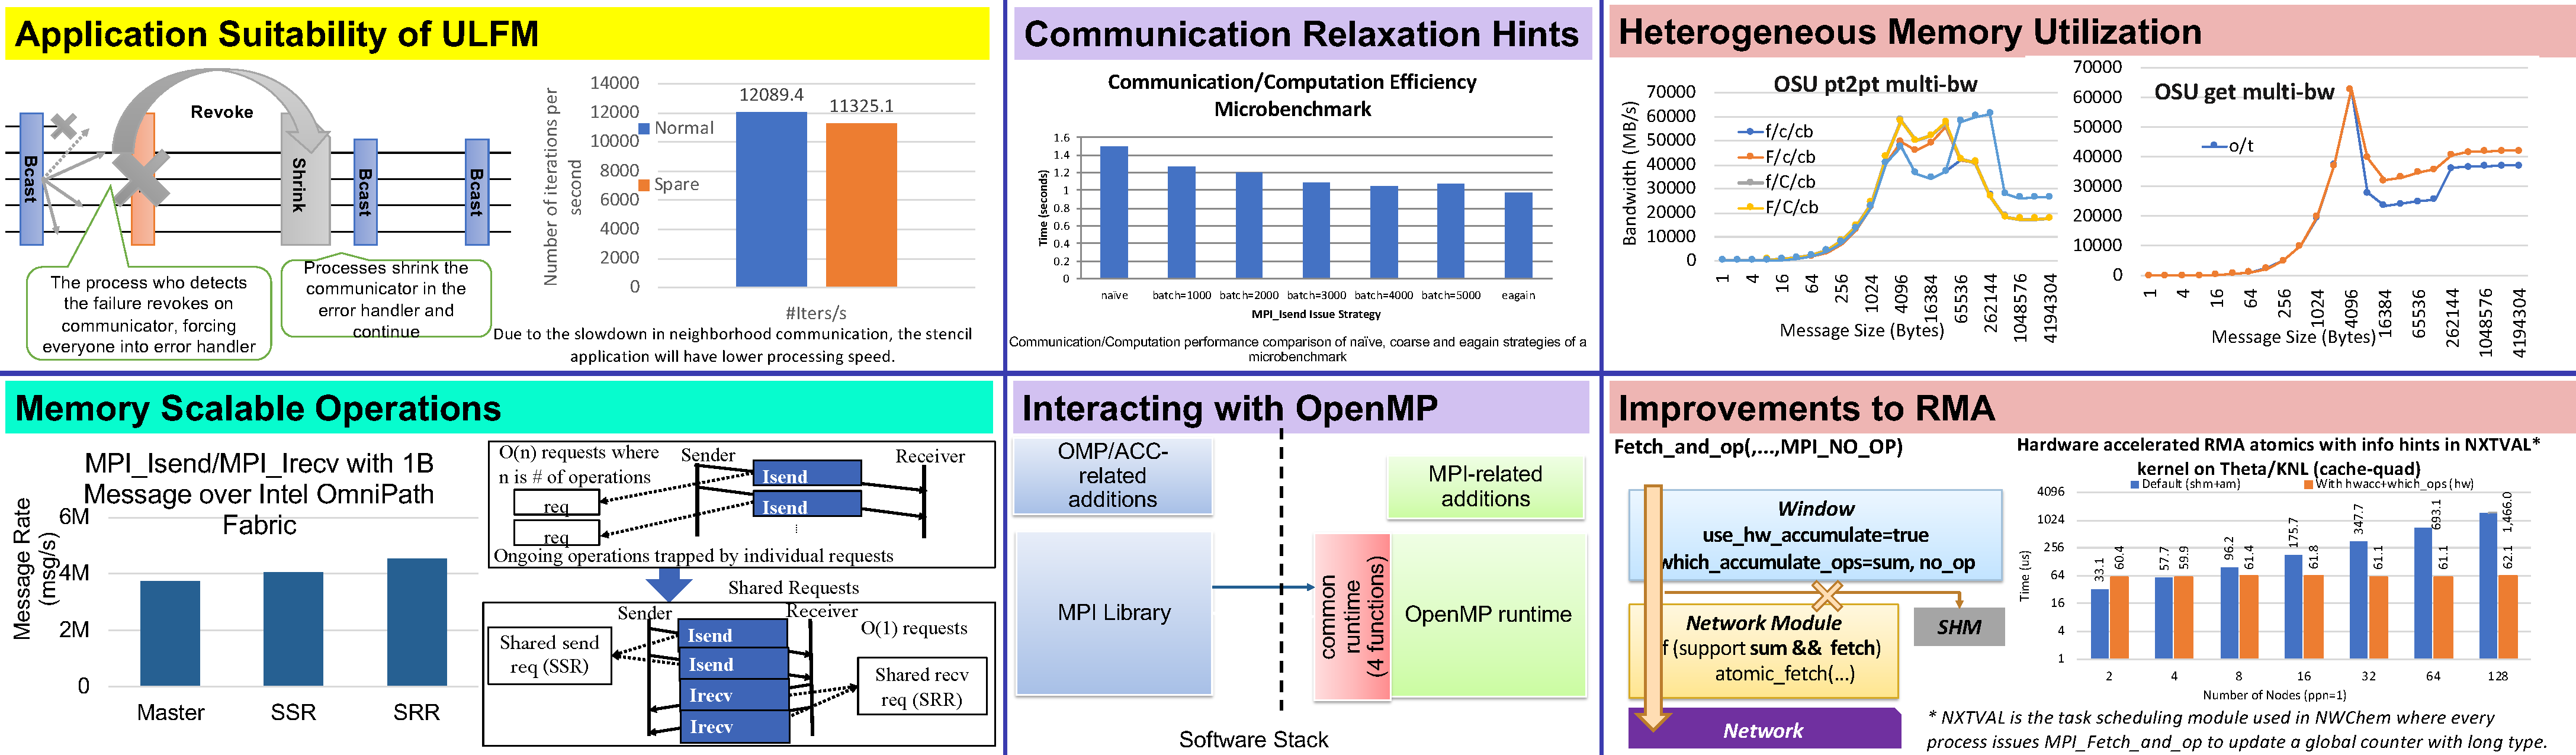
\includegraphics[width=6in]{projects/2.3.1-PMR/2.3.1.07-Exascale-MPI/MPICH-recent-milestones.pdf}
  \caption{\label{fig:sep18}MPICH milestones
    completed in June 2018 and Septmeber 2018}
\end{figure}

In the first milestone completed in September 2018, lightweight send and receive requests
for communication are instroduced. In this
way, we are able to only use constant number of requests to track many operations which
significantly reduce the memory scalability
of MPI. Furthermore, by sharing the preallocated requests, we also avoid the costs
of request allocation and initialization within each operation and achieved even higher message rate.
In the second milestone completed in September 2018, introduced MPI info, "disable\_shm\_accumulate",
to only use network-based atomics for MPI accumulates in specific windows and
"which\_accumulate\_ops", to limit the need of atomic support at runtime.

\paragraph{Next Steps}
Exascale MPI ongoing efforts include ECP application performance evaluation of utilizing
heterogeneous memory inside the MPI implementation, analysis of the performance evaluation
of the implementation of virtual topology functionality, standardization of ULFM
in MPI and finally, investigate and evaluate the implementation of MPI-4 ULFM proposal in MPICH,
to investigate a study of the benefit potential of the MPI endpoints approach and evaluate
it with selected ECP applications and to investigate
topology-aware collectives and neighborhood collectives in MPICH and evaluate the selected ECP applications.

\newpage
\input{projects/2.3.1-PMR/2.3.1.08-Legion/2.3.1.08-Legion}
\clearpage
\newpage
\input{projects/2.3.1-PMR/2.3.1.09-ParSEC/2.3.1.09-ParSEC}
\newpage
\input{projects/2.3.1-PMR/2.3.1.10-Kokkos-Support/2.3.1.10-Kokkos-Support}
\newpage
\input{projects/2.3.1-PMR/2.3.1.11-OMPI-X/2.3.1.11-OMPI-X}
\newpage
\input{projects/2.3.1-PMR/2.3.1.12-Power-Steering/2.3.1.12-Power-Steering}
\newpage
\input{projects/2.3.1-PMR/2.3.1.13-SOLLVE/2.3.1.13-SOLLVE}
\newpage
\input{projects/2.3.1-PMR/2.3.1.13-SOLLVE/2.3.1.13-SOLLVE-ARGOBOTS}
\newpage
\input{projects/2.3.1-PMR/2.3.1.13-SOLLVE/2.3.1.13-SOLLVE-BOLT}
\newpage
\input{projects/2.3.1-PMR/2.3.1.14-UPCxx-GASNet/2.3.1.14-UPCxx}
\newpage
\input{projects/2.3.1-PMR/2.3.1.14-UPCxx-GASNet/2.3.1.14-GASNet-EX}
\newpage
\input{projects/2.3.1-PMR/2.3.1.15-Qthreads/2.3.1.15-Qthreads}
\newpage
\input{projects/2.3.1-PMR/2.3.1.16-SICM/2.3.1.16-SICM}
\newpage

\subsection{\tools}
This section present projects in \tools.
\newpage
\input{projects/2.3.2-Tools/2.3.2.01-Tools-SDKs/2.3.2.01-Tools-SDKs}
\newpage
\input{projects/2.3.2-Tools/2.3.2.02-LANL-ATDM-Tools/2.3.2.02-LANL-ATDM-Tools}
\newpage
\input{projects/2.3.2-Tools/2.3.2.03-LLNL-ATDM-Tools/2.3.2.03-LLNL-ATDM-Tools}
\newpage
\input{projects/2.3.2-Tools/2.3.2.04-SNL-ATDM-Tools/2.3.2.04-SNL-ATDM-Tools}
\newpage
\input{projects/2.3.2-Tools/2.3.2.05-Exascale-Code-Generation-Toolkit/2.3.2.05-Exascale-Code-Generation-Toolkit}
\newpage
\input{projects/2.3.2-Tools/2.3.2.06-EXA-PAPI/2.3.2.06-EXA-PAPI}
\newpage
\input{projects/2.3.2-Tools/2.3.2.07-Autotuning/2.3.2.07-Autotuning}
\newpage
\input{projects/2.3.2-Tools/2.3.2.08-HPCToolkit/2.3.2.08-HPCToolkit}
\newpage
\input{projects/2.3.2-Tools/2.3.2.09-PROTEAS/2.3.2.09-PROTEAS}
\newpage
\input{projects/2.3.2-Tools/2.3.2.09-PROTEAS/2.3.2.09-TAU}
\newpage
\input{projects/2.3.2-Tools/2.3.2.09-PROTEAS/2.3.2.09-PAPYRUS}
\newpage
\input{projects/2.3.2-Tools/2.3.2.09-PROTEAS/2.3.2.09-CLACC}
\newpage

\subsection{\mathlibs}
This section present projects in \mathlibs.
\newpage
\input{projects/2.3.3-MathLibs/2.3.3.01-xSDK/2.3.3.01-xSDK}
\newpage
\input{projects/2.3.3-MathLibs/2.3.3.01-xSDK/2.3.3.01-xSDK-hypre}
\newpage
\input{projects/2.3.3-MathLibs/2.3.3.02-LANL-ATDM-MathLibs/2.3.3.02-LANL-ATDM-MathLibs}
\newpage
\input{projects/2.3.3-MathLibs/2.3.3.03-LLNL-ATDM-MathLibs/2.3.3.03-LLNL-ATDM-MathLibs}
\newpage
\subsubsection{\stid{3.04} ATDM SNL Math Libraries} \label{subsubsect:trilinos}

\paragraph{Overview} 
The major project outcome for the SNL ATM Math Libraries project is to provide re-usable and convenient, math-related tools for component-based software engineering of Exascale apps.

This project develops and integrates scalable, modular, and cross-cutting software infrastructure components for ATDM and other future Exascale applications that utilize, where appropriate, ATDM Core CS components: Kokkos performance portability, Sacado/ROL embedded sensitivity analysis and optimization technology, DARMA asynchronous many-tasking, and DataWarehouse.  These components include:
\begin{enumerate}
\item	KokkosKernels (KK):  performance-portable sparse/dense linear algebra and graph kernels that utilize the hierarchical memory subsystem expected in future architectures;
\item	Scalable Solvers (SS):  optimal linear solver algorithms that exploit fine-grain parallelism for vector/SIMT and thread scaling and leverage next-generation execution and communication capabilities;
\item	Agile Components (AC):  tools for interface abstractions, discretization, time integration, and solution of nonlinear PDEs; and 
\item Embedded Analysis (EA):  tools for enabling advanced analysis workflows, focusing on embedded sensitivity analysis and optimization with use of derivatives for uncertainty quantification.
\end{enumerate}

This project combines algorithmic R\&D with delivery of interoperable software components that are expected to be crucial capabilities that will enable Sandia's ATDM application codes to be performance portable across next-generation computing architectures such as GPUs and Xeon Phis.  This work will include integration of these components into the application codes and improving their design and interfaces for mission relevant use cases.	


\paragraph{Key  Challenges}
There are several challenges associated with the work this project is conducting. Part of the complexity arises because profiling tools are not yet full mature for advanced architectures and in this context profiling involves the interplay of several factors which require expert judgment to improve performance.  Another challenging aspect is working on milestones that span a variety of projects and code bases. There is a strong dependence on the various application code development teams for our own team's success. In addition, we face a constant tension between the need for production ready tools and components in a realm where the state-of-the-art is still evolving.

\paragraph{Solution Strategy}
To address the challenges above, the SNL ATM Math Libraries project is taking a staged approach to profiling in regards to target architectures and the algorithms involved. We are also coordinating on a regular basis with the other projects that are involved in our work to minimize impediments. In response to the need for production ready tools, we are focusing on a hierarchical approach that involves producing robust, hardened code for core algorithms while simultaneous pursuing research ideas where appropriate.

\paragraph{Recent Progress}
In this section we provide several high-level snapshots of recent progress in the Math Libraries project
\begin{itemize}
\item The SS team has recently achieved 10 solves/sec for the miniEM proxy application for EMPIRE, this is important for meeting the efficiency requirements to complete upcoming milestones.
\item The SS team is also making good progress in identifying other performance bottlenecks, such as over-decomposition. We now have performance date supporting hypotheses like these.
\item the AC team is working to promote CUDA aware GPU/GPU transfers in Tpetra.
\item the KK team made a recent presentation to Jim Peltz on the features of KK and recent progress.
\item The EA team has made progress in terms of addressing Stokhos issues that were holding up Kokkos promotion.
\item The AC team has made implemented a hierarchical parallelism approach to some of the kernels in Panzer leading to significant speedup.
\item the KK team finished work on SIMD with the University of Utah and submitted a paper on how to use SIMD in three cases.
\end{itemize}

\paragraph{Next Steps}
The following list details the next steps being taking by each component of the ATDM SNL Math Libraries project:

\begin{itemize}
\item The KK team is investigating using dynamic sizing for batched BLAS.
\item The SS team is continuing to investigate, in collaboration with the University of Wyoming, the use of Multilevel solvers, which will eventually get integrated into SPARC via MueLu.
\item The AC is continuing to work on the integration of Tempus into EMPIRE-PIC, including enabling higher order integration schemes.
\item The EA team is working on enabling transient full space optimization in SPARC.

\end{itemize}

\newpage
\input{projects/2.3.3-MathLibs/2.3.3.05-SUNDIALS/2.3.3.05-SUNDIALS}ZZ
\newpage
\subsubsection{\stid{3.06} PETSc-TAO} \label{subsubsect:petsc}
\paragraph{Overview} 

Algebraic solvers (generally nonlinear solvers that use sparse linear solvers via Newton's method) and ODE/DAE 
integrators form the core computation of many numerical simulations. No scalable ``black box'' sparse solvers 
or integrators work for all applications, nor single implementations that work well for all scales of 
problem size. Hence, algebraic solver packages provide a wide variety of algorithms and implementations 
that can be customized for the application and range of problem sizes at hand. PETSc~\cite{petsc:homepage,petsc-man} 
is a widely used software library for the scalable solution of linear, nonlinear, and ODE/DAE systems and 
computation of adjoints (sometimes called sensitivities) of ODE systems. We focus on three topics: (1) partially 
matrix-free scalable solvers efficiently use many-core and GPU-based systems; (2) reduced synchronization 
algorithms that can scale to larger concurrency than solvers with synchronization points; and (3) performance 
and data structure optimizations for all the core data structures to better utilize many-core and GPU-based 
systems as well as provide scalability to the Exascale.

The availability of systems with over 100 times the processing power of today's machines compels the utilization 
of these systems not just for a single ``forward solve'' simulation (as discussed above) but rather within a 
tight loop of optimization, sensitivity analysis (SA), and uncertain quantification (UQ). This requires the 
implementation of a new, scalable library for managing a dynamic hierarchical collection of running scalable simulations, where the simulations directly feed results into the optimization, SA, and UQ solvers.  This library, 
which we call libEnsemble, directs the multiple concurrent ``function evaluations'' through the tight coupling 
and feedback described above. This work consist of two parts: (1) the development of libEnsemble and (2) the 
extension of TAO~\cite{tao-man} (our PETSc-based scalable optimization library) with new algorithms and 
software to utilize libEnsemble.

\paragraph{Key Challenges}

A key challenge for for scaling the PETSc/TAO numerical libraries to Exascale systems is that 
traditional ``sparse-matrix-based'' techniques for linear, nonlinear, and ODE solvers, as well 
as optimization algorithms, are memory-bandwidth limited.  Another difficulty is that any 
synchronizations required across all compute units--for example, an inner product or a 
norm--can dramatically affect the scaling of the solvers.

Running an ensemble of simulation requires a coordination layer that handles load balancing and
allows the collection of running simulations to grow and shrink based on feedback. Thus, this 
library must be able to dynamically start simulations with different parameters, resume 
simulations to obtain more accurate results, prune running simulations that the solvers 
determine can no longer provide useful information, monitor the progress of the simulations, 
and stop failed or hung simulations, and collect data from the individual simulations both 
while they are running and at the end.

\paragraph{Solution Strategy}

To address the scalability of the numerical libraries, we are developing new solvers and data 
structures including pipeline Krylov methods that delay the use of the results of inner products 
and norms, allowing overlapping of the reductions and other computation; partially matrix-free 
solvers using high-order methods that have high floating-point-to-memory-access ratios and
good potential to use many-core and GPU-based systems; and in-node optimizations of sparse 
matrix-matrix products needed by algebraic multigrid to better utilize many-core systems
using a thread neutral ``bypass MPI'' approach, which implements default interprocessor 
communication using MPI but bypasses the use of MPI in performance-critical regions 
for higher performance and thereby maintains MPI portability.

Our strategy for coordinating ensemble computations has been to develop libEnsemble
to satisfy our needs.  This library should not be confused with workflow-based 
scripting systems; rather it is a library that, through the tight coupling and 
feedback described above, directs the multiple concurrent ``function evaluations''
needed by optimization, SA, and UQ solvers.

\paragraph{Recent Progress}

In the past year, we have released PETSc 3.10 (available at \url{http://www.mcs.anl.gov/petsc})
that features enhanced GPU support.  In particular, PETSc’s algebraic multigrid (AMG) consists 
of two main components: the setup (coarsening) phase which has both GPU and CPU intensive 
portions and the solve stage which can run largely or completely on the GPU. A key 
requirement is minimizing the amount of communication needed between the CPU 
and GPU during both phases of the computation.  In the PETSc~3.10 release, we 
completed porting key AMG kernels for both phases to GPUs via CUDA, enabling
this code to run on a combination of the CPU and GPU.

\begin{figure}
\centering
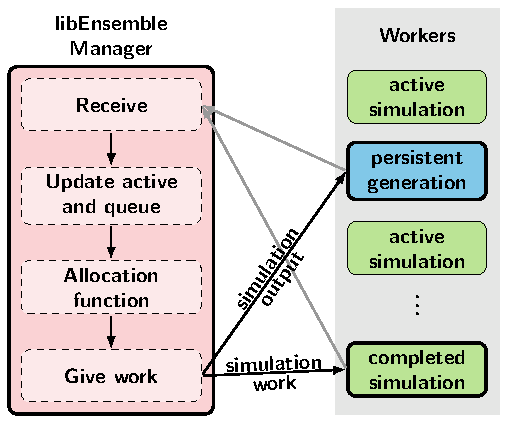
\includegraphics[width=0.5\textwidth]{projects/2.3.3-MathLibs/2.3.3.06-PETSc-TAO/lib_ensemble}
\caption{The libEnsemble control flow showing a manager coordinating workers executing 
calculations of either simulation functions or generation functions.}
\label{fig:petsc-tao-fig}
\end{figure}

We have also developed the libEnsemble API, implemented it in Python, released 
version 0.4 (available at \url{https://github.com/Libensemble/libensemble}),
and provided a Spack installation.

\paragraph{Next Steps}

Our next efforts are:
\begin{enumerate}
  \item \textbf{Release libEnsemble with active management capabilities}: Add active management 
    capabilities into libEnsemble to set precision of the simulation and to store information 
    from simulations to evaluate objectives as they evolve. Work with application teams to 
    determine requirements on libEnsemble and provide assistance in its usage.
  \item \textbf{Release PETSc/TAO with optimized support for LCF machines and ECP applications}:
    Work with application teams to provide assistance in PETSc/Tao usage. Provide optimizations 
    based on application profiling.
\end{enumerate}


\newpage
\input{projects/2.3.3-MathLibs/2.3.3.07-STRUMPACK-SuperLU/2.3.3.07-STRUMPACK-SuperLU}
\newpage
\input{projects/2.3.3-MathLibs/2.3.3.08-ForTrilinos/2.3.3.08-ForTrilinos}
\newpage
\subsubsection{\stid{3.09} SLATE}\label{subsubsect:slate}


\paragraph{Overview}

The Software for Linear Algebra Targeting Exascale (SLATE) intends to
provide fundamental dense linear algebra capabilities
to the US Department of Energy (DOE)
and to the high-performance computing (HPC) community at large.
To this end, SLATE will provide
parallel Basic Linear Algebra Subprograms (BLAS),
linear systems solvers, least square solvers,
singular value and eigenvalue solvers.

The ultimate objective of SLATE is to replace the
venerable Scalable Linear Algebra PACKage (ScaLAPACK) library,
which has become the industry standard for dense linear algebra operations
in distributed-memory environments.
However, after two decades of operation,
ScaLAPACK is past the end of its life cycle and overdue for a replacement,
as it can hardly be retrofitted to support GPUs,
which are an integral part of today's HPC hardware infrastructure.

Primarily, SLATE aims to extract the full performance potential and maximum
scalability from modern HPC machines with large numbers nodes,
large numbers of cores per node, and multiple GPUs per node.
For typical dense linear algebra workloads, this means getting close
to the theoretical peak performance and scaling to the full size of the machine
(i.e., thousands to tens of thousands of nodes).
This is to be accomplished in a portable manner by relying mostly on standards
like MPI and OpenMP.

SLATE functionalities will first be delivered to the ECP applications
that most urgently require SLATE capabilities
(NWChem, GAMESS, EXAALT, QMCPACK, CANDLE, etc.)
and to other software libraries
that rely on underlying dense linear algebra services
(STRUMPACK, SuperLU, etc.).
Figure~\ref{fig:slate-architecture} shows the role of SLATE
in the ECP software stack.

While the initial objective of SLATE is to serve as a successful,
drop-in replacement for ScaLAPACK with support for GPU accelerators,
the ultimate goal of SLATE is to deliver dense linear algebra capabilities
way beyond the capabilities of ScaLAPACK.
The low-hanging fruits include implementation of more communication-avoiding
algorithms and randomization algorithms
(based on random projections and sampling).
Also within the reach of SLATE are features like:
support for variable size tiles, support for low-rank compressed tiles,
and possibly support for block-sparse matrices.

\begin{figure}[htb]
    \centering
    \includegraphics[width=0.75\textwidth]{projects/2.3.3-MathLibs/2.3.3.09-SLATE/SLATE-architecture.jpg}
    \caption{\label{fig:slate-architecture}
    SLATE in the ECP software stack.}
\end{figure}

\paragraph{Key  Challenges}

\begin{enumerate}
\item
\textbf{Designing from the ground up:}
The SLATE project's primary challenge stems from the need to design the package
from the ground up, as no existing software package offers
a viable path forward for efficient support of GPUs
in a distributed-memory environment.
\item
\textbf{Facing harsh hardware realities:}
SLATE is being developed in a harsh hardware environment, where virtually
all the processing power is on the GPU side.
Achieving efficiency requires very aggressive offload to GPU accelerators
and very careful optimization of multiple bottlenecks.
Being a distributed computing package, SLATE also faces the grim reality
of the interconnection technology lagging horribly behind the computing
capabilities of the GPUs.
\item
\textbf{Facing harsh software realities:}
SLATE is being developed using cutting-edge software technologies,
and relies on modern features of the C++ language and recent extensions
to the OpenMP standard, many of which are not fully supported by compilers
and their runtime environments.
In terms of GPU acceleration, standardized solutions are still in flux.
Also, while complete parallel programming frameworks exist, at this stage
they have to be considered research prototypes.
\end{enumerate}

\paragraph{Solution Strategy}

\begin{enumerate}
\item
\textbf{Evolving design:}
Due to the inherent challenges of designing a software package
from the ground up, the SLATE project started
with a careful analysis of the existing and emerging
implementation technologies~\cite{abdelfattah2017roadmap},
and followed with a phase
of laying out the initial design~\cite{kurzak2017designing}.
Since then, the team rolls out new computational routines every quarter,
while frequently refactoring and occasionally redesigning the underlying
software infrastructure.
\item
\textbf{Focus on GPUs:}
Efficient GPU acceleration is the primary focus of performance
engineering efforts in SLATE.
Where applicable, highly optimized vendor implementations of GPU operations
are used, such as the batch {\tt gemm} routine.
Where necessary, custom GPU kernels are developed, like in the case of computing
matrix norms.
Care is taken to hide communication to and from the GPUs by overlapping it with
execution of GPU computations.
\item
\textbf{Community engagement:}
The SLATE team interact on a regular basis with the OpenMP community,
represented in ECP by the SOLLVE project, and with the MPI community,
represented in ECP by the OMPI-X project and the Exascale MPI project.
The SLATE team also engages the vendor community through our contacts
at Intel, NVIDIA, AMD, and ARM.
\end{enumerate}

\paragraph{Recent Progress}

During each quarter of 2018, the SLATE team has been adding to its suite
by releasing new computational routines:
parallel Level 3 BLAS in March,
parallel norms in June,
linear systems solvers (LLT, LU, LDLT) in September,
and least squares solvers (CAQR/LQ) in December.
All routines are available in all standard precisions:
single real (S), single complex (C), double real (D), and double complex (Z),
all accompanied by appropriate testers.
In addition to SLATE's native, C++ API, compatibility APIs for LAPACK
and ScaLAPACK users are also provided, so that SLATE can serve
as a drop-replacement.
All developments are documented in SLATE Working Notes
\footnote{\url{http://www.icl.utk.edu/publications/series/swans}.}

\paragraph{Next Steps}

\begin{enumerate}
\item
\textbf{Mixed-precision Linear Solvers:}
We plan to implement mixed-precision linear solvers by the end of March 2019.
Mixed precision routines factor the matrix in lower precision, e.g., single,
and compute the linear system solution in higher precision, e.g., double,
in the process of iterative refinement.
In most cases, results in the high precision can be produced at the speed
of computing in the low precision.
The half precision of the Tensor Cores of the V100 GPUs are a possible target
of this technique.
\item
\textbf{Matrix Inversion Routines:}
We plan to implement matrix inversion routines by the end of June 2019.
Explicit matrix inverses are required by applications in computational
chemistry and statistics, and offer a high potential for optimization
by pipelining the different algorithmic steps.
Routines for inverting general, symmetric positive definite, and symmetric
indefinite matrices are planned.
\item
\textbf{SVD and EVP Solvers:}
We plan to implement SVD routines and symmetric EVP routines
by the end of September 2019.
The implementations will be based on state-of-the-art two-stage reductions
and divide-and-conquer algorithms.
Superior performance is expected, as well as strong benefit
from GPU acceleration.
\end{enumerate}

\newpage
\input{projects/2.3.3-MathLibs/2.3.3.10-PEEKS/2.3.3.10-PEEKS}
\newpage
\subsubsection{\stid{3.11} ALExa}


\paragraph{Overview}

The ALExa project ({\sl Accelerated Libraries for Exascale}) focuses on
preparing the DTK and Tasmanian libraries for exascale platforms and
integrating these libraries into ECP applications.  These libraries deliver
capabilities identified as needs of ECP applications: (1) the ability to
transfer computed solutions between grids with differing layouts on parallel
accelerated architectures, enabling multiphysics projects to seamlessly
combine results from different computational grids to perform their required
simulations (DTK); and
%
(2) the ability to construct fast and memory efficient surrogates to large
scale engineering models with multiple inputs and large number of outputs,
enabling uncertainty quantification (both forward and inverse) as well as
optimization and efficient multi-physics simulations in projects such as
ExaStar (Tasmanian).

These capabilities are being developed through ongoing interactions with our
ECP application project collaborators to ensure they will satisfy requirements
of these customers.  The libraries in turn take advantage of other ECP/SW
capabilities currently in development, including Trilinos and ForTrilinos,
Kokkos and SLATE.  The final outcome of the ECP project will be a set of
libraries deployed to facilities and also made broadly available as part of
the xSDK4ECP project.


{\bf DTK} (Data Transfer Kit)

{\it Purpose:} Transfers computed solutions between grids with differing
layouts on parallel accelerated architectures.

{\it Significance:} Coupled applications frequently have different grids with
different parallel distributions; DTK is able to transfer solution values
between these grids efficiently and accurately.

{\it Mesh and mesh-free interpolation capabilities:} multivariate data
interpolation between point clouds and grids; compactly supported radial basis
functions; nearest-neighbor and moving least square implementations; support
for standard finite-element shape functions and user-defined interpolants;
common applications include conjugate heat transfer, fluid structure
interaction, and mesh deformation.

{\it Performance portable search capabilities:} shared memory and GPU
implementations of spatial tree construction; shared memory and GPU
implementations of various spatial tree queries; MPI front-end for
coordinating distributed spatial searches between sets of geometric objects
with different decompositions; communication plan generation based on spatial
search results.

{\it URL:} https://github.com/ORNL-CEES/DataTransferKit


{\bf Tasmanian} (Toolkit for Adaptive Stochastic Modeling and Non-Intrusive
Approximation)

{\it Purpose:} Constructs efficient surrogate models for high dimensional
problems and performs parameter calibration and optimization geared towards
applications in uncertainty quantification (UQ).

{\it Significance:} UQ pertains to the statistical properties of the output
from a complex model with respect to variability in multiple model inputs;
large number of simulations are required to compute reliable statistics which
is prohibitive when dealing with computationally expensive engineering
models. A surrogate model is constructed from a moderate set of simulations
using carefully chosen input values; analysis can then be performed on the
efficient surrogate.

{\it Sparse grids capabilities:} surrogate modeling and design of experiments
(adaptive multi-dimensional interpolation); reduced (lossy) representation of
tabulated scientific data; high dimensional numerical quadrature; data mining
and manifold learning.

{\it DiffeRential Evolution Adaptive Metropolis (DREAM) capabilities:}
Bayesian inference; parameter estimation/calibration; model validation.
global optimization and optimization under uncertainty.

{\it URL:} http://tasmanian.ornl.gov

\paragraph{Key Challenges}

\indent

{\bf DTK:} General data transfer between grids of unrelated applications
requires many-to-many communication which is increasingly challenging as
communication to computation ratios are decreasing on successive HPC systems.
Search procedures to locate neighboring points and mesh cells require tree
search methods difficult to optimize on modern accelerated architectures due
to vector lane or thread divergence. Maintaining high accuracy for the
transfer requires careful attention to the mathematical properties of the
interpolation methods and is highly application-specific.

{\bf Tasmanian:} Complex models usually have significant variability in
execution time for different model inputs, which leads to massive down-time
when employing the standard fork-join adaptive sparse grid algorithms.  After
the surrogate has been constructed, collecting the samples for statistical
analysis (or multi-physics simulations) requires a massive number of basis
evaluations and many sparse and dense linear operations.

\paragraph{Solution Strategy}

\nobreak


\indent

{\bf DTK:} State-of-the-art, mathematically rigorous methods are used in DTK
to preserve accuracy of interpolated solutions.  Algorithms are implemented in
a C++ code base with extensive unit testing on multiple platforms.  Trilinos
packages are used to support interpolation methods.  Kokkos is used to achieve
performance portability across accelerated platforms.

{\bf Tasmanian:} Implement asynchronous DAG-based sparse grids construction
methods that preserve the convergence properties of the fork-join algorithms
but are insensitive to fluctuations in model simulation time.  Port the basis
evaluations and linear algebra to the GPU accelerators, and leverage the
SLATE/MAGMA capabilities to ensure performance portability across relevant
platforms.


%----------------------------------------

\paragraph{Recent Progress}

\indent

{\bf DTK:} Extensive optimization work has yielded significant performance
improvements on accelerated and heterogeneous architectures. Work with partner
application ExaAM (WBS 2.2.1.05) created a preliminary multiphysics driver
capability for additive manufacturing simulations.

\begin{figure}[htb]
        \centering
        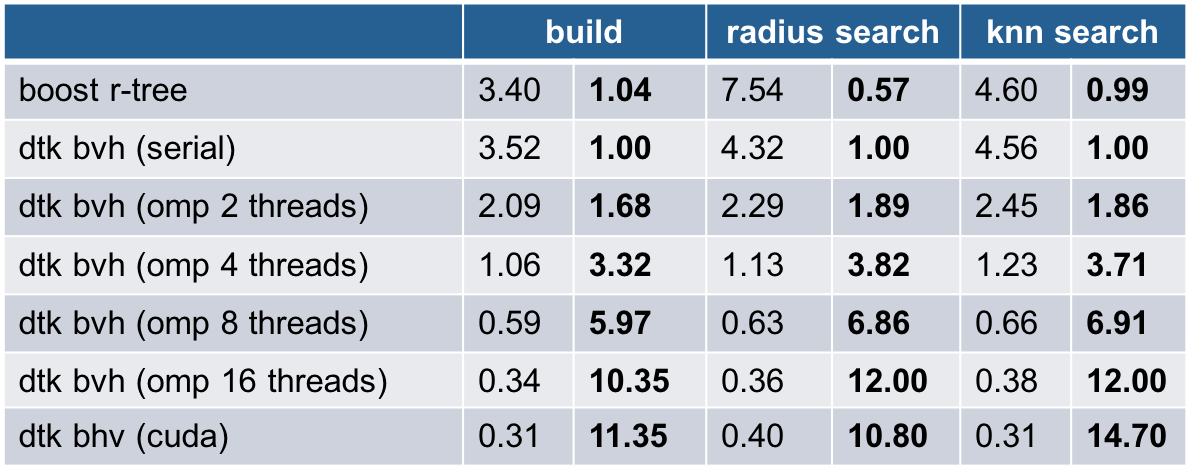
\includegraphics[width=3.0in]{projects/2.3.3-MathLibs/2.3.3.11-ALExa/dtk-gpu}
        \caption{\label{fig:dtk-gpu}DTK search performance relative to Boost with Intel Xeon E5-2698 and Nvidia P100. 10M points randomly distributed in a unit cube, 1M queries. The time is in seconds. Speedup in bold.}
\end{figure}

{\bf Tasmanian:} The infrastructure of Tasmanian has been upgraded to support
the broader ECP focus of the work.  GPU acceleration of sparse grid surrogates
has been implemented.  Tasmanian recently enabled the ExaStar project to
reduce the size of a large-memory table of neutrino opacities by 100X while
still preserving accuracy.

\begin{figure}[htb]
        \centering
        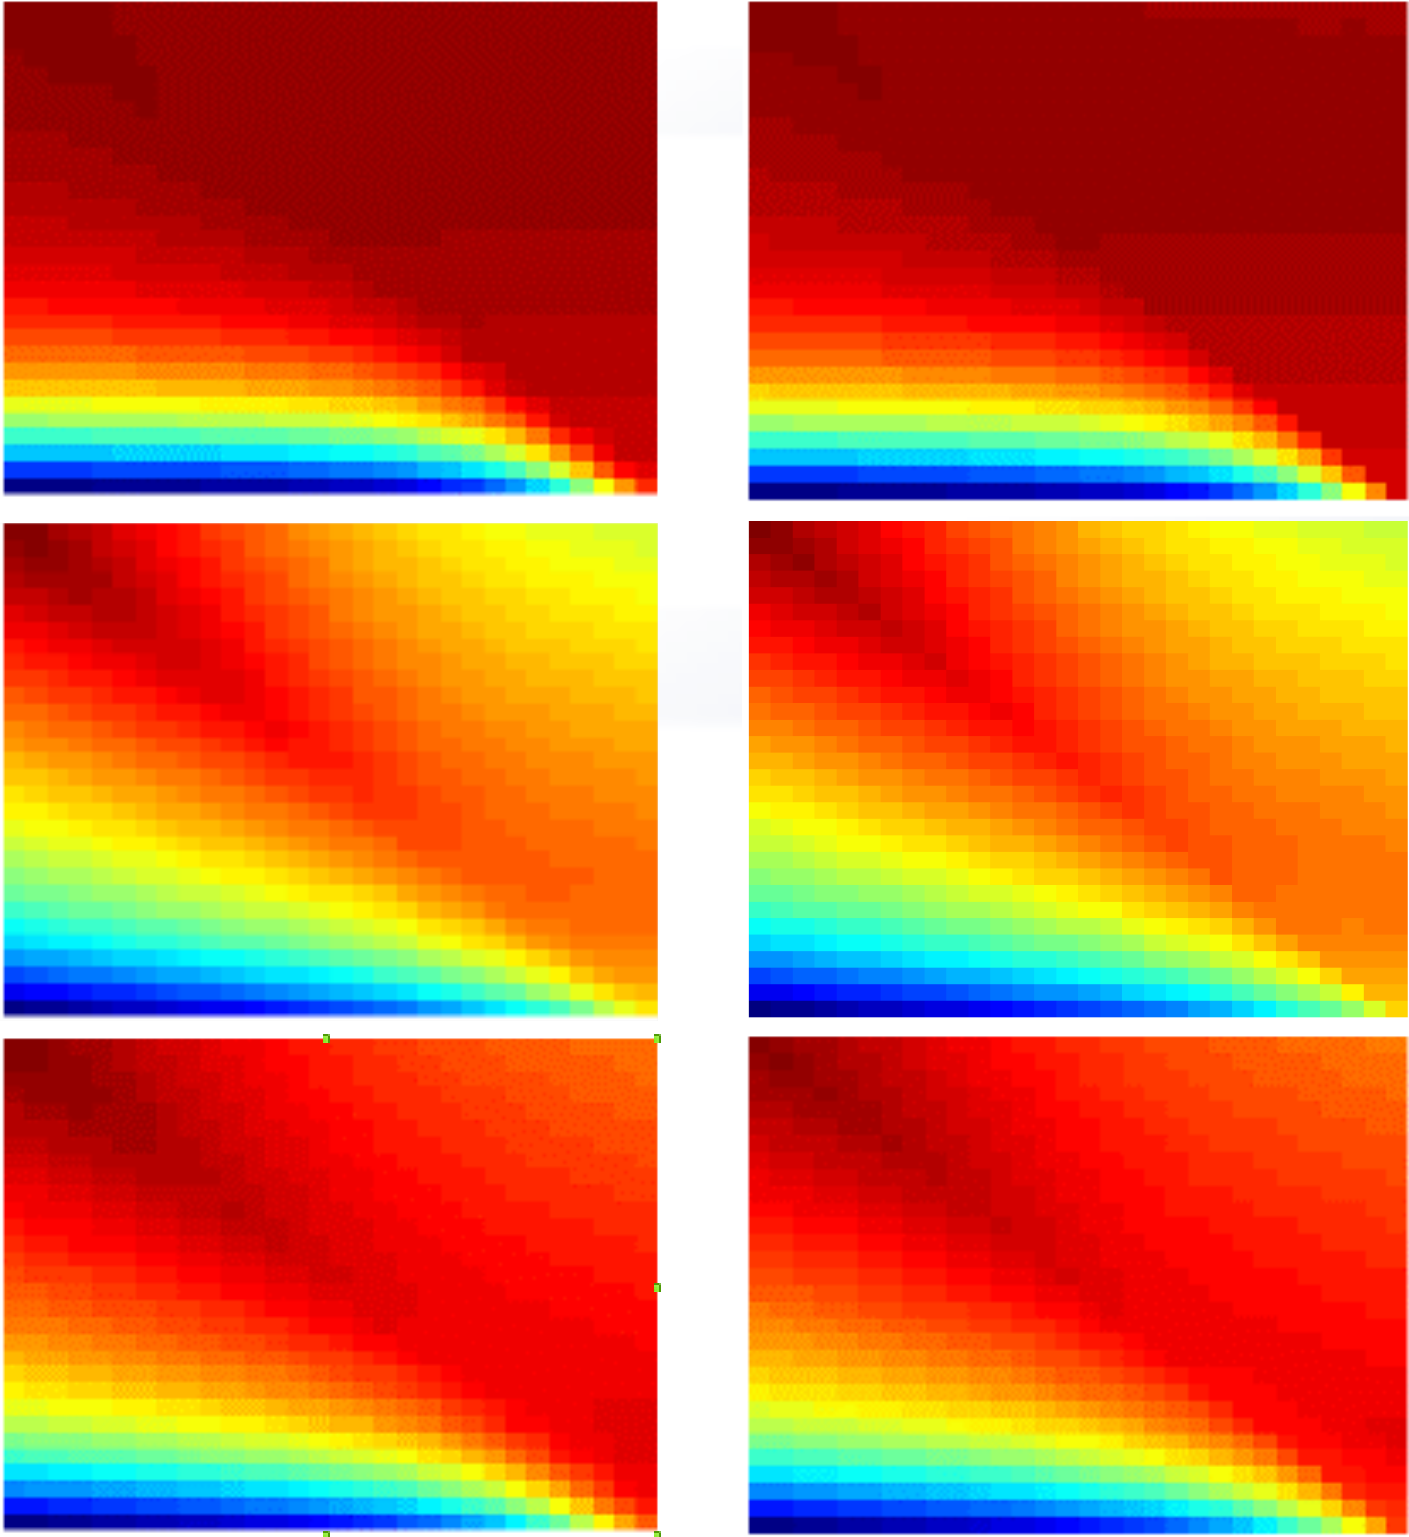
\includegraphics[width=1.5in]{projects/2.3.3-MathLibs/2.3.3.11-ALExa/tasmanian-gpu}
        \caption{\label{fig:tasmanian-gpu}Tasmanian approximation (right) of neutrino capacities (left).}
\end{figure}

%----------------------------------------

\paragraph{Next Steps}

\indent

{\bf DTK:} DTK search and communication capabilities will deployed in a new,
lightweight library, ArborX, to provide these ECP investments to a broader
user base.

{\bf Tasmanian:} Work will continue with the development of the asynchronous
construction methods that exploit the native sparse grids DAG hierarchy.

%----------------------------------------

\newpage

\subsection{\dataviz}
This section present projects in \dataviz.
\newpage
\input{projects/2.3.4-DataViz/2.3.4.01-DataViz-SDK/2.3.4.01-DataViz-SDK}
\newpage
\input{projects/2.3.4-DataViz/2.3.4.02-LANL-ATDM-DataViz/2.3.4.02-LANL-ATDM-DataViz}
\newpage
\input{projects/2.3.4-DataViz/2.3.4.03-LLNL-ATDM-DataViz/2.3.4.03-LLNL-ATDM-DataViz}
\newpage
\input{projects/2.3.4-DataViz/2.3.4.04-SNL-ATDM-DataViz/2.3.4.04-SNL-ATDM-Data}
\newpage
\input{projects/2.3.4-DataViz/2.3.4.04-SNL-ATDM-DataViz/2.3.4.04-SNL-ATDM-Viz}
\newpage
\input{projects/2.3.4-DataViz/2.3.4.05-VeloC/2.3.4.05-VeloC}
\newpage
\input{projects/2.3.4-DataViz/2.3.4.06-EZ/2.3.4.06-EZ}
\newpage
\input{projects/2.3.4-DataViz/2.3.4.07-UNIFYCR/2.3.4.07-UNIFYCR}
\newpage
\input{projects/2.3.4-DataViz/2.3.4.08-ExaHDF5/2.3.4.08-ExaHDF5}
\newpage
\input{projects/2.3.4-DataViz/2.3.4.09-ADIOS/2.3.4.09-ADIOS}
\newpage
\input{projects/2.3.4-DataViz/2.3.4.10-DataLib/2.3.4.10-DataLib}
\newpage
\input{projects/2.3.4-DataViz/2.3.4.11-ZFP/2.3.4.11-ZFP}
\newpage
\input{projects/2.3.4-DataViz/2.3.4.12-ALPINE/2.3.4.12-ALPINE}
\newpage
% -*- latex -*-

\subsubsection{\stid{4.13} ECP/VTK-m}

\paragraph{Overview}
The ECP/VTK-m project is providing the core capabilities to perform scientific visualization on Exascale architectures.
The ECP/VTK-m project fills the critical feature gap of performing visualization and analysis on processors like graphics-based processors and many integrated core.
The results of this project will be delivered in tools like ParaView, VisIt, and Ascent as well as in stand-alone form.
Moreover, these projects are depending on this ECP effort to be able to make effective use of ECP architectures.

One of the biggest recent changes in high-performance computing is the increasing use of accelerators.
Accelerators contain processing cores that independently are inferior to a core in a typical CPU, but these cores are replicated and grouped such that their aggregate execution provides a very high computation rate at a much lower power.

Current and future CPU processors also require much more explicit parallelism.
Each successive version of the hardware packs more cores into each processor, and technologies like hyper threading and vector operations require even more parallel processing to leverage each core's full potential.

VTK-m is a toolkit of scientific visualization algorithms for emerging processor architectures.
VTK-m supports the fine-grained concurrency for data analysis and visualization algorithms required to drive extreme scale computing by providing abstract models for data and execution that can be applied to a variety of algorithms across many different processor architectures.

The ECP/VTK-m project is building up the VTK-m codebase with the necessary visualization algorithm implementations that run across the varied hardware platforms to be leveraged at the Exascale.
We will be working with other ECP projects, such as ALPINE, to integrate the new VTK-m code into production software to enable visualization on our HPC systems.

\paragraph{Key  Challenges}
The scientific visualization research community has been building scalable HPC algorithms for over 15 years, and today there are multiple production tools that provide excellent scalability.
However, our current visualization tools are based on a message-passing programming model.
More to the point, they rely on a coarse decomposition with ghost regions to isolate parallel execution \cite{Ahrens2001,Childs2010}.
However, this decomposition works best when each processing element has on the order of a hundred thousand to a million data cells \cite{ParaViewTutorial} and is known to break down as we approach the level of concurrency needed on modern accelerators \cite{Moreland2012:Ultravis,Moreland2013:UltraVis}.

DOE has made significant investments in HPC visualization capabilities.
For us to feasibly update this software for the upcoming Exascale machines, we need to be selective on what needs to be updated, and we need to maximize the code we can continue to use.
Regardless, there is a significant amount of software to be engineered and implemented, so we need to extend our development resources by simplifying algorithm implementation and providing performance portability across current and future devices.


\paragraph{Solution Strategy}
The ECP/VTK-m project leverages VTK-m \cite{Moreland2016:VTKm} to overcome these key challenges.
VTK-m has a software framework that provides the following critical features.

\begin{enumerate}
\item \textbf{Visualization building blocks:}
  VTK-m contains the common data structures and operations required for scientific visualization.
  This base framework simplifies the development of visualization algorithms \cite{VTKmUsersGuide}.
\item \textbf{Device portability:}
  VTK-m uses the notion of an abstract device adapter, which allows algorithms written once in VTK-m to run well on many computing architectures.
  The device adapter is constructed from a small but versatile set of data parallel primitives, which can be optimized for each platform \cite{Blelloch1990}.
  It has been shown that this approach not only simplifies parallel implementations, but also allows them to work well across many platforms \cite{Lo2012,Larsen2015,Moreland2015}.
\item \textbf{Flexible integration:}
  VTK-m is designed to integrate well with other software.
  This is achieved with flexible data models to capture the structure of applications' data \cite{Meredith2012} and array wrappers that can adapt to target memory layouts \cite{Moreland2012:PDAC}.
\end{enumerate}

Even with these features provided by VTK-m, we have a lot of work ahead of us to be ready for Exascale.
Our approach is to incrementally add features to VTK-m and expose them in tools like ParaView and VisIt.


\begin{figure}[t]
  \centering
  \includegraphics[width=2in]{projects/2.3.4-DataViz/2.3.4.13-ECP-VTK-m/VTKm-Multiblock}\quad
  \includegraphics[width=2in]{projects/2.3.4-DataViz/2.3.4.13-ECP-VTK-m/VTKm-Gradients}\quad
  \includegraphics[width=2in]{projects/2.3.4-DataViz/2.3.4.13-ECP-VTK-m/VTKm-FieldToColors}
  \caption{
    Examples of recent progress in VTK-m include (from left to right) multiblock data structures, gradient estimation, and mapping of fields to colors.
  }
  \label{fig:VTKmRecent}
\end{figure}

\paragraph{Recent Progress}
The VTK-m project is organized into many implementation activities.
The following features have been completed in the FY18 fiscal year.

\begin{itemize}
\item \textbf{Multiblock Data:}
  Treat multiple blocks of data, such as those depicted in Figure \ref{fig:VTKmRecent} at left, as first-class data sets.
  %Direct support of multiblock data not only provides programming convenience but also allows us to improve scheduling tasks for smaller groups of data.
\item \textbf{Gradients:}
  Gradients, depicted in Figure \ref{fig:VTKmRecent} at center, are an important metric of fields and must often be derived using topological data.
  %Gradients are also fundamental in finding important vector field qualities like divergence, vorticity, and q-criterion.
\item \textbf{Field to Colors:}
  Pseudocoloring, demonstrated in Figure \ref{fig:VTKmRecent} at right, is a fundamental feature of scientific visualization, and it depends on a good mechanism of converting field data to colors.
\item \textbf{VTK-m 1.1 Release:}
  VTK-m 1.1 was released in December 2017.
\item \textbf{Extract External Surface:}
  When rendering solid objects, it is only necessary to render the external surface of the object as the interior of the volume is hidden \cite{Lessley2016,Lessley2017}.
  %As such, external surface extraction is one of the most common operations in scientific visualization applications.
\item \textbf{Coordinate system transformations:}
  3D rendering systems operate in Cartesian coordinate systems.
  However, data are sometimes referenced in cylindrical or spherical coordinate systems.% to match the physical structure of the data.
  %Consequently, visualization tools need a fast method to convert coordinates among different spaces.
\item \textbf{Affine Transformations:}
  Affine transformations, which include translate, rotate, and scale, are a common and important method to manipulate objects in 3D space.
\item \textbf{Location Structures:}
  Finding mesh components from a coordinate in space requires search structures.
\item \textbf{Rendering Topological Entities:}
  It is often helpful to analysts to view representations of the constitute components of a mesh.
\item \textbf{OpenMP:}
  %Much of the code we wish to integrate with uses OpenMP \cite{OpenMP}, which can conflict with other threading implementations.
  %VTK-m now supports multiple threading libraries, including OpenMP, to better match the code it integrates with.
  VTK-m now supports OpenMP \cite{OpenMP} to better match the code it integrates with.
\end{itemize}

\paragraph{Next Steps}
Our next efforts include:

\begin{itemize}
\item \textbf{Dynamic Types:}
  %The initial implementation of VTK-m used templating to adjust to different data structures.
  %However, when data types are not known at compile time, which is common in applications like ParaView and VisIt, templating for all possible combinations becomes infeasible.
  Provide mechanisms to enable runtime polymorphism.
\item \textbf{ZFP:}
  We are assisting the ZFP project (WBS 2.3.4.11) by helping them implement {\zfp} in VTK-m and port across ECP platforms.
\item \textbf{Clip:}
  Cuts away a mesh based on a spatial intersection or field values.
\item \textbf{Ghost Cells:}
  Provide better support for ghost/halo regions across blocks in a mesh.
\item \textbf{Merge Points:}
  Combine points in a mesh that can be considered coincident.
\item \textbf{Connected Components:}
  Identify regions in a mesh where all cells are topologically connected to each other.
\item \textbf{Particle Advection:}
  Many flow visualization algorithms depend on computing the movement of weightless particles in a flow vector field.
%% \item \textbf{Lightweight Cell Library:}
%%   There is much repetition between VTK-m and other visualization code to perform operations on cells.
%%   We would like to consolidate that code into a lightweight library.
\end{itemize}

\noindent
{\tiny Sandia National Laboratories is a multimission laboratory managed and operated by National Technology \& Engineering Solutions of Sandia, LLC, a wholly owned subsidiary of Honeywell International Inc., for the U.S. Department of Energy's National Nuclear Security Administration under contract DE-NA0003525. \hfill SAND~2018-13745~R
\par}

\newpage

\subsection{\ecosystem}
This section present projects in \ecosystem.
\newpage
\input{projects/2.3.5-Ecosystem/2.3.5.01-Ecosystem-SDK/2.3.5.01-Ecosystem-SDK}
\newpage
\input{projects/2.3.5-Ecosystem/2.3.5.02-LANL-ATDM-Ecosystem/2.3.5.02-LANL-ATDM-Ecosystem}
\newpage
\input{projects/2.3.5-Ecosystem/2.3.5.03-LLNL-ATDM-Ecosystem/2.3.5.03-LLNL-ATDM-Ecosystem}
\newpage
\input{projects/2.3.5-Ecosystem/2.3.5.04-SNL-ATDM-Ecosystem/2.3.5.04a-SNL-ATDM-Ecosystem}
\newpage
\input{projects/2.3.5-Ecosystem/2.3.5.04-SNL-ATDM-Ecosystem/2.3.5.04b-SNL-ATDM-Ecosystem}
\newpage
\input{projects/2.3.5-Ecosystem/2.3.5.05-Argo/2.3.5.05-Argo}
\newpage
\input{projects/2.3.5-Ecosystem/2.3.5.06-Flang/2.3.5.06-Flang}

\newpage
\section{Conclusion}

ECP ST is providing a collection of essential software capabilities necessary for successful results from Exascale computing platforms, while also delivery a suite of products that can be sustained into the future.  This Capabilities Assessment Report and subsequent versions will provide a periodic summary of capabilities, plans, and challenges as the Exascale Computing Project proceeds.
%%---------------------------------------------------------------------------%%
\newpage
\section*{Acknowledgements}

This research was supported by the Exascale Computing Project (ECP), Project
Number: 17-SC-20-SC, a collaborative effort of two DOE organizations---the
Office of Science and the National Nuclear Security
Administration---responsible for the planning and preparation of a capable
Exascale ecosystem---including software, applications, hardware, advanced
system engineering, and early testbed platforms---to support the nation's
Exascale computing imperative.

%%---------------------------------------------------------------------------%%
%% References
\newpage
\bibliographystyle{unsrt}
\bibliography{references,projects/2.3.1-PMR/2.3.1.01-PMR-SDKs/2.3.1.01-PMR-SDKs,projects/2.3.1-PMR/2.3.1.02-LANL-ATDM-PMR/2.3.1.02-LANL-ATDM-PMR,projects/2.3.1-PMR/2.3.1.03-LLNL-ATDM-PMR/2.3.1.03-LLNL-ATDM-PMR,projects/2.3.1-PMR/2.3.1.05-Global-Arrays/2.3.1.05-Global-Arrays,projects/2.3.1-PMR/2.3.1.06-RAJA/2.3.1.06-RAJA,projects/2.3.1-PMR/2.3.1.07-Exascale-MPI/2.3.1.07-Exascale-MPI,projects/2.3.1-PMR/2.3.1.08-Legion/2.3.1.08-Legion,projects/2.3.1-PMR/2.3.1.09-ParSEC/2.3.1.09-ParSEC,projects/2.3.1-PMR/2.3.1.11-OMPI-X/2.3.1.11-OMPI-X,projects/2.3.1-PMR/2.3.1.12-Power-Steering/2.3.1.12-Power-Steering,projects/2.3.1-PMR/2.3.1.13-SOLLVE/2.3.1.13-SOLLVE,projects/2.3.1-PMR/2.3.1.13-SOLLVE/2.3.1.13-SOLLVE-ARGOBOTS,projects/2.3.1-PMR/2.3.1.13-SOLLVE/2.3.1.13-SOLLVE-BOLT,projects/2.3.1-PMR/2.3.1.14-UPCxx-GASNet/2.3.1.14-UPCxx,projects/2.3.1-PMR/2.3.1.14-UPCxx-GASNet/2.3.1.14-GASNet-EX,projects/2.3.1-PMR/2.3.1.15-Qthreads/2.3.1.15-Qthreads,projects/2.3.1-PMR/2.3.1.16-SICM/2.3.1.16-SICM,projects/2.3.2-Tools/2.3.2.01-Tools-SDKs/2.3.2.01-Tools-SDKs,projects/2.3.2-Tools/2.3.2.02-LANL-ATDM-Tools/2.3.2.02-LANL-ATDM-Tools,projects/2.3.2-Tools/2.3.2.03-LLNL-ATDM-Tools/2.3.2.03-LLNL-ATDM-Tools,projects/2.3.2-Tools/2.3.2.04-SNL-ATDM-Tools/2.3.2.04-SNL-ATDM-Tools,projects/2.3.2-Tools/2.3.2.05-Exascale-Code-Generation-Toolkit/2.3.2.05-Exascale-Code-Generation-Toolkit,projects/2.3.2-Tools/2.3.2.06-EXA-PAPI/2.3.2.06-EXA-PAPI,projects/2.3.2-Tools/2.3.2.07-Autotuning/2.3.2.07-Autotuning,projects/2.3.2-Tools/2.3.2.08-HPCToolkit/2.3.2.08-HPCToolkit,projects/2.3.2-Tools/2.3.2.09-PROTEAS/2.3.2.09-PROTEAS,projects/2.3.2-Tools/2.3.2.09-PROTEAS/2.3.2.09-TAU,projects/2.3.2-Tools/2.3.2.09-PROTEAS/2.3.2.09-PAPYRUS,projects/2.3.2-Tools/2.3.2.09-PROTEAS/2.3.2.09-CLACC,projects/2.3.3-MathLibs/2.3.3.01-xSDK/2.3.3.01-xSDK,projects/2.3.3-MathLibs/2.3.3.01-xSDK/2.3.3.01-xSDK-hypre,projects/2.3.3-MathLibs/2.3.3.02-LANL-ATDM-MathLibs/2.3.3.02-LANL-ATDM-MathLibs,projects/2.3.3-MathLibs/2.3.3.03-LLNL-ATDM-MathLibs/2.3.3.03-LLNL-ATDM-MathLibs,projects/2.3.3-MathLibs/2.3.3.04-SNL-ATDM-MathLibs/2.3.3.04-SNL-ATDM-MathLibs,projects/2.3.3-MathLibs/2.3.3.05-SUNDIALS/2.3.3.05-SUNDIALS,projects/2.3.3-MathLibs/2.3.3.06-PETSc-TAO/2.3.3.06-PETSc-TAO,projects/2.3.3-MathLibs/2.3.3.07-STRUMPACK-SuperLU/2.3.3.07-STRUMPACK-SuperLU,projects/2.3.3-MathLibs/2.3.3.08-ForTrilinos/2.3.3.08-ForTrilinos,projects/2.3.3-MathLibs/2.3.3.09-SLATE/2.3.3.09-SLATE,projects/2.3.3-MathLibs/2.3.3.10-PEEKS/2.3.3.10-PEEKS,projects/2.3.3-MathLibs/2.3.3.11-ALExa/2.3.3.11-ALExa,projects/2.3.4-DataViz/2.3.4.01-DataViz-SDK/2.3.4.01-DataViz-SDK,projects/2.3.4-DataViz/2.3.4.02-LANL-ATDM-DataViz/2.3.4.02-LANL-ATDM-DataViz,projects/2.3.4-DataViz/2.3.4.03-LLNL-ATDM-DataViz/2.3.4.03-LLNL-ATDM-DataViz,projects/2.3.4-DataViz/2.3.4.04-SNL-ATDM-DataViz/2.3.4.04-SNL-ATDM-Data,projects/2.3.4-DataViz/2.3.4.04-SNL-ATDM-DataViz/2.3.4.04-SNL-ATDM-Viz,projects/2.3.4-DataViz/2.3.4.05-VeloC/2.3.4.05-VeloC,projects/2.3.4-DataViz/2.3.4.06-EZ/2.3.4.06-EZ,projects/2.3.4-DataViz/2.3.4.07-UNIFYCR/2.3.4.07-UNIFYCR,projects/2.3.4-DataViz/2.3.4.09-ADIOS/2.3.4.09-ADIOS,projects/2.3.4-DataViz/2.3.4.11-ZFP/2.3.4.11-ZFP,projects/2.3.4-DataViz/2.3.4.12-ALPINE/2.3.4.12-ALPINE,projects/2.3.4-DataViz/2.3.4.13-ECP-VTK-m/2.3.4.13-ECP-VTK-m,projects/2.3.5-Ecosystem/2.3.5.01-Ecosystem-SDK/2.3.5.01-Ecosystem-SDK,projects/2.3.5-Ecosystem/2.3.5.02-LANL-ATDM-Ecosystem/2.3.5.02-LANL-ATDM-Ecosystem,projects/2.3.5-Ecosystem/2.3.5.03-LLNL-ATDM-Ecosystem/2.3.5.03-LLNL-ATDM-Ecosystem,projects/2.3.5-Ecosystem/2.3.5.04-SNL-ATDM-Ecosystem/2.3.5.04-SNL-ATDM-Ecosystem,projects/2.3.5-Ecosystem/2.3.5.05-Argo/2.3.5.05-Argo,projects/2.3.5-Ecosystem/2.3.5.06-Flang/2.3.5.06-Flang}

%%---------------------------------------------------------------------------%%
%% APPENDIX
%%---------------------------------------------------------------------------%%
% The ECP ST CAR Appendix is kept in a private repo.  It must be cloned/forked and be side-by-side with the ECP-ST-CAR-PUBLIC repo if the following line is uncommented.
%\input{../ECP-ST-CAR-APPENDIX/appendix}

\end{document}
